% Autor: Dominik Harmim <harmim6@gmail.com>

\documentclass[a4paper, 10pt, twocolumn]{article}

\usepackage[czech]{babel}
\usepackage[utf8]{inputenc}
\usepackage[T1]{fontenc}
\usepackage[left=2cm, top=2cm, text={17cm, 25cm}]{geometry}
\usepackage[unicode, colorlinks, hypertexnames=false, citecolor=red]{hyperref}
\usepackage{times}
\usepackage{graphicx}
\usepackage{amsmath}


\begin{document}
    \twocolumn[
        \begin{@twocolumnfalse}
            \begin{center}
                {\Large
                    Vysoké učení technické v~Brně \\
                    Fakulta informačních technologií \\
                }
                {
\includegraphics[width=.4 \linewidth]{img/FIT_logo.pdf}} \\

                {\LARGE
                    Paralelní a~distribuované algoritmy \\
                    2. Projekt\,--\,Odd-Even Transposition Sort \\[.4cm]
                }

                {\large
                    Dominik Harmim (xharmi00) \\
                    \texttt{xharmi00@stud.fit.vutbr.cz} \\
                    \today
                }
            \end{center}
        \end{@twocolumnfalse}
    ]


    \section{Rozbor algoritmu}

    Algoritmus \emph{Odd-Even Transposition Sort} je \emph{paralelní řadící
    algoritmus}, který předpokládá \emph{lineární pole procesů}. Dále se
    budeme bavit o~verzi algoritmu, který řadí prvky \emph{vzestupně}.

    Pro seřazení~$ n $~hodnot je potřeba~$ n $~procesů. Předpokládá se,
    že sousední procesy spolu mohou komunikovat. Na počátku každý
    proces~$ p_i $~obsahuje jednu z~řazených hodnot~$ x_i $. V~prvním kroku
    algoritmu každý \emph{lichý proces}~$ p_i $~porovná svoji
    hodnotu~$ x_i $~s~hodnotou~$ x_{i - 1} $~svého levého
    souseda~$ p_{i - 1} $~a~pokud je jeho hodnota menší než hodnota souseda
    ($ x_i < x_{i - 1} $), procesy své hodnoty vymění. V~druhém kroku
    provedou analogickou operaci všechny \emph{sudé procesy}. Řazené hodnoty
    budou seřazeny nanejvýše po~$ n $~takovýchto krocích, kde se střídají
    sudé a~liché procesy. Obrázek~\ref{fig:algorithm-demo} demonstruje
    fungování tohoto algoritmu.

    \begin{figure}[ht]
        \centering
        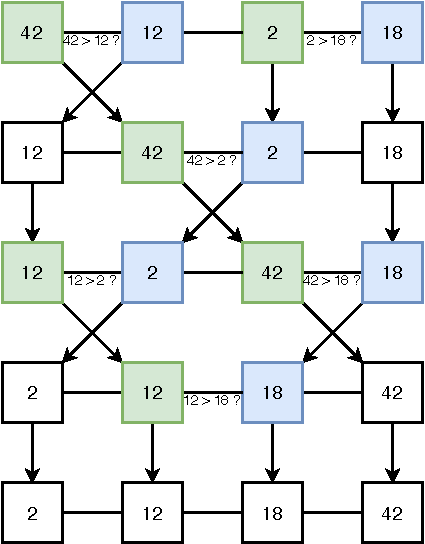
\includegraphics[width=.6 \linewidth]{img/algorithm-demo.pdf}
        \caption{Demonstrace řazení prvků algoritmem}
		\label{fig:algorithm-demo}
    \end{figure}

    \subsection{Analýza algoritmu}

    Jak již bylo řečeno výše, počet procesů pro seřazení~$ n $~prvků
    je~$ n $, tedy $ p(n) = n $.

    Každý proces si vždy pamatuje hodnotu právě jednoho prvku.
    \emph{Prostorová složitost} je proto~$ n $, tedy $ s(n) = n $.

    V~každém kroku algoritmu se provádí paralelně na každém druhém procesu
    jedno porovnání a~dva přenosy hodnot. \emph{Časová složitost} je tedy
    konstantní, $ t(n) = \mathcal{O}(n) $.

    \emph{Celková cena} tohoto algoritmu je následující: $ c(n) = t(n) \cdot
    p(n) = \mathcal{O}(n) \cdot n = \mathcal{O}(n^2) $. Tato cena
    \emph{není optimální}, protože $ \mathcal{O}(n^2) \neq \mathcal{O}(
    n \cdot \log n) $, kde $ \mathcal{O}(n \cdot \log n) $ je cena
    optimálního sekvenčního řadícího algoritmu.

    \emph{Zrychlení} tohoto algoritmu oproti optimálnímu sekvenčnímu řeší,
    který má časovou složitost $ t(n) = \mathcal{O}(n \cdot \log n) $, je
    následující: $ \frac{\mathcal{O}(n \cdot \log n)}{\mathcal{O}(n)} =
    \mathcal{O}(\log n) $.


    \section{Implementace}

    Algoritmus je implementován v~programovacím jazyce C++. Je využito
    knihovny \emph{Open MPI} pro zasílání zpráv mezi procesy. Implementace
    se nachází v~souboru \texttt{ots.cpp}. Po spuštění programu se hned
    po inicializaci knihovny Open MPI zjistí číslo procesu, které mu
    knihovna přidělila. Podle tohoto čísla se potom rozhoduje, jak se
    bude daný proces chovat a~se kterými procesy bude komunikovat
    (rozdělení na sudé/liché procesy). Procesy se číslují přirozenými čísly
    včetně čísla~0. Proces s~číslem~0, tzv. hlavní proces, je proces, který
    provádí vstupní a~výstupní operace a~který iniciuje komunikace
    s~ostatními procesy a~celou komunikaci řídí. Lze říci, že program je
    rozdělen do 3 částí, které budou dále blíže popsány.

    V~1.~části programu provádí hlavní proces funkci \texttt{read\_numbers},
    která čte řazené prvky (konkrétně přirozená čísla včetně
    čísla~0~v~rozsahu 0-255) ze vstupního souboru \texttt{numbers} a~tyto
    vypisuje na standardní výstup a~následně je postupně posílá všem procesům
    včetně sebe samotného (počet procesů musí být roven počtu čísel ve
    vstupním souboru, což je zajištěno při spouštění programu připraveným
    testovacím skriptem \texttt{test.sh}). Zasíláním a~přijímáním prvků
    od procesů se bude dále myslet dvojice knihovních funkcí
    \texttt{MPI\_Send}/\texttt{MPI\_Recv}. Všechny ostatní procesy volají
    funkci \texttt{receive\_number} (i~hlavní proces po zpracování vstupního
    souboru), kde přijímají řazený prvek od hlavního procesu, který se tímto
    stane jejich prvkem.

    Ve 2.~části programu probíhá samotné řazení prvků. Toto je implementováno
    funkcí \texttt{ots}. Zde se $ m $-krát, kde $ m =
    \frac{\text{počet procesů}}{2} $, provádí paralelní porovnávání nejdříve
    lichých procesů a~následně paralelní porovnávání sudých procesů.
    Porovnání probíhá tím způsobem, že proces zašle sousednímu procesu
    prvek a~čeká na přijetí nového prvku. Sousední proces nový prvek
    spočítá tím způsobem, že přijatý prvek porovná se svým prvek a~v~případě
    potřeby je prohodí a~prvek zašle zpátky sousedovi.

    Ve 3.~části programu všechny procesy kromě hlavního procesu posílají
    své prvky hlavnímu procesu. Hlavní proces všechny prvky přijímá
    a~ukládá si je do pomocného pole. Toto se děje ve funkci
    \texttt{receive\_all\_numbers}. Po přijetí všech prvků je postupně
    tiskne na standardní výstup funkcí \texttt{print\_numbers}.

    Na obrázku~\ref{fig:seq-diagram} je sekvenční diagram, který znázorňuje
    výše popsanou komunikaci mezi procesy.

    \begin{figure}[ht]
        \centering
        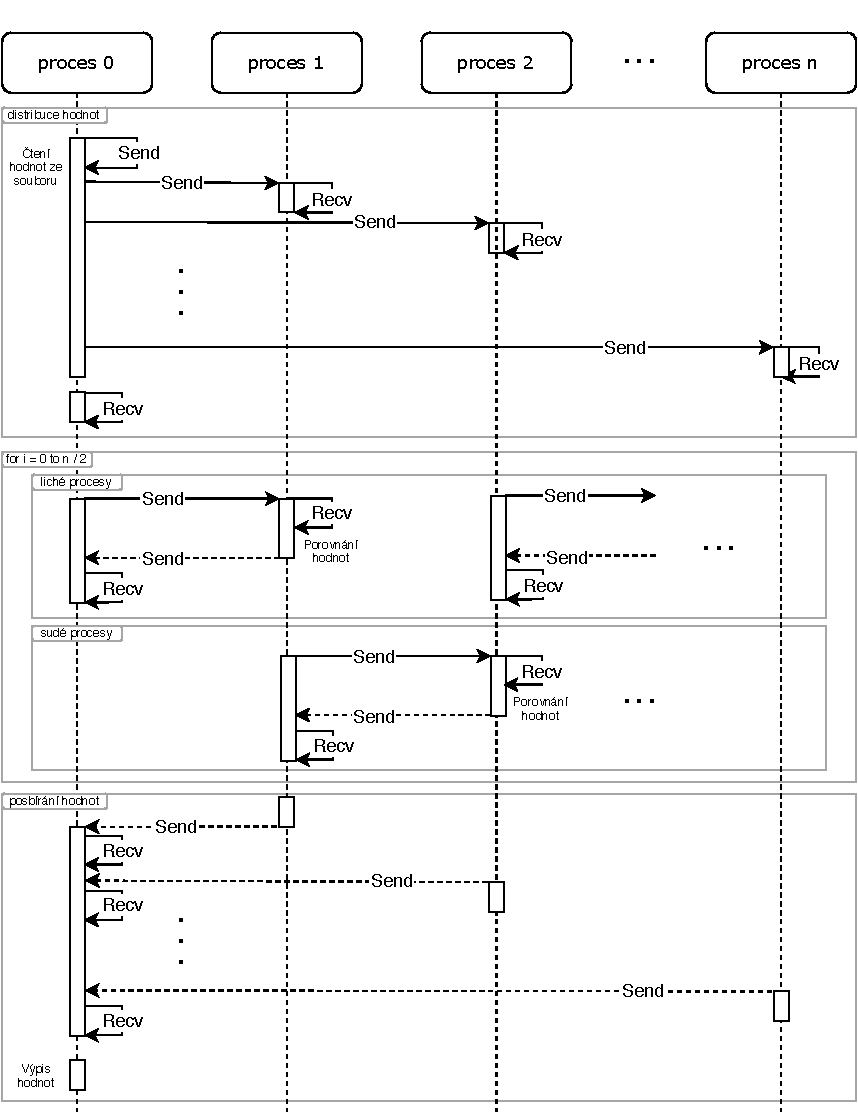
\includegraphics[width=.95 \linewidth]{img/sequence-diagram.pdf}
        \caption{Komunikační protokol procesů}
		\label{fig:seq-diagram}
    \end{figure}


    \section{Experimenty}

    Pro ověření teoretické časové složitosti byly provedeny experimenty,
    kde byl měřen reálný čas provádění řazení prvků funkcí
    \texttt{std::chrono::high\_resolution\_clock::now}. Měření bylo prováděno
    na stroji, kde je možné spustit nanejvýše přibližně~100 procesů, proto
    bylo měření provedeno nejvýše se~100 prvky. Měření bylo provedeno pro
    různý počet prvků od~5 až do~100 prvků. Každé měření pro určitý počet
    prvků bylo prováděno několikrát a~výsledky byly průměrovány, aby nebyly
    vidět případné odchylky. Výsledky tohoto měření jsou k~vidění na
    obrázku~\ref{fig:experiments}. Je vidět, že reálná časová složitost roste
    přibližně lineárně, stejně jako teoretická.

    \begin{figure}[ht]
        \centering
        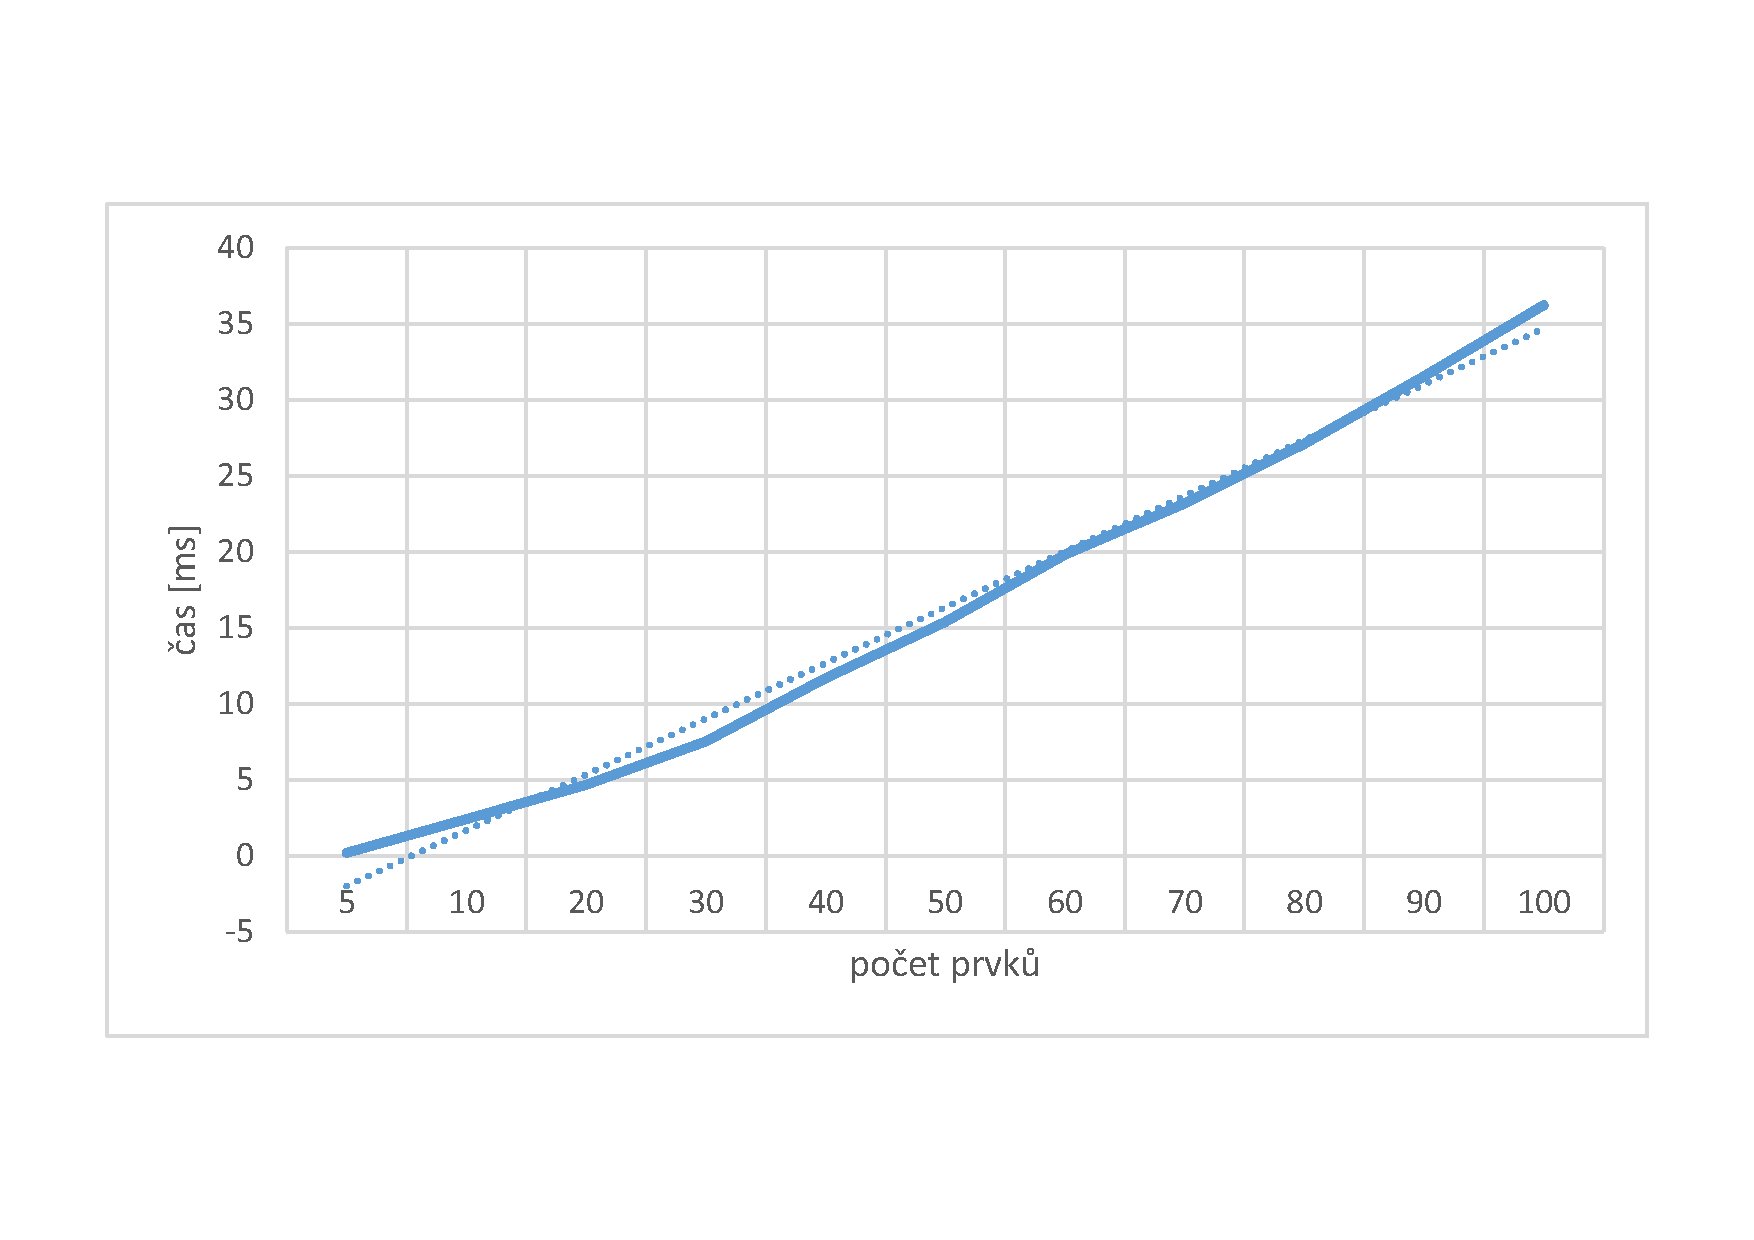
\includegraphics[width=1 \linewidth]{img/experiments.pdf}
        \caption{Výsledky měření experimentů}
		\label{fig:experiments}
    \end{figure}


    \section{Závěr}

    V~rámci tohoto projekty byla úspěšně vytvořena implementace algoritmu
    Odd-Even Transposition Sort. Teoretický časová složitost tohoto
    algoritmu byla ověřena reálnými experimenty.
\end{document}
